\documentclass{article}

% if you need to pass options to natbib, use, e.g.:
%     \PassOptionsToPackage{numbers, compress}{natbib}
% before loading neurips_2020

% ready for submission
% \usepackage{neurips_2020}

% to compile a preprint version, e.g., for submission to arXiv, add add the
% [preprint] option:
%     \usepackage[preprint]{neurips_2020}

% to compile a camera-ready version, add the [final] option, e.g.:
%     \usepackage[final]{neurips_2020}

% to avoid loading the natbib package, add option nonatbib:
\usepackage[preprint, nonatbib]{neurips_2020}

\usepackage[utf8]{inputenc} % allow utf-8 input
\usepackage[T1]{fontenc}    % use 8-bit T1 fonts
\usepackage{hyperref}       % hyperlinks
\usepackage{url}            % simple URL typesetting
\usepackage{booktabs}       % professional-quality tables
\usepackage{amsfonts}       % blackboard math symbols
\usepackage{nicefrac}       % compact symbols for 1/2, etc.
\usepackage{microtype}      % microtypography\usepackage{amsmath}
\usepackage{stmaryrd}
\usepackage{multirow}
\usepackage{xcolor}
\usepackage[pdftex]{graphicx}
\usepackage{multirow}
\usepackage{tabularx} 
\usepackage{array}
\usepackage[justification=centering]{caption}
\usepackage{amsmath}

\newcolumntype{P}[1]{>{\centering\arraybackslash}p{#1}}
\newcolumntype{M}[1]{>{\centering\arraybackslash}m{#1}}

\usepackage{stfloats}
% declare the path(s) where your graphic files are
\graphicspath{{figures/}}

\usepackage[sorting=none]{biblatex}
\addbibresource{citations/citations.bib}
\addbibresource{citations/dnn.bib}

\title{Project Report:\\Fast and Memory-Efficient Coarse-Grained Audio Classification using Deep Neural Network}

\author{
Md Shamim Hussain\\
Department of Computer Science\\
Rensselaer Polytechnic Institute\\
110 8th St.\\ Troy, NY, USA\\
\texttt{hussam4@rpi.edu} \\
\And
Nafis Neehal\\
Department of Computer Science\\
Rensselaer Polytechnic Institute\\
110 8th St.\\ Troy, NY, USA\\
\texttt{neehan@cs.rpi.edu} \\
}

\begin{document}

\maketitle

\begin{abstract}
  Deep neural networks are notorious for their high computational cost and memory requirements. Not only that, often they need specialized hardware for efficient execution. However, for simple tasks such as a coarse-grained classification of sound into superclasses such as speech, music, and noise, one may not be able to spare a lot of computational resources. In this work, we devise a new convolutional network - SwishNetV2 which is fast and memory-efficient, but gets close to big convolutional networks such as VGG16 in terms of classification performance. This architecture improves upon the previous SwishNet architecture and performs well on the CPU with limited memory requirements, similar to its predecessor. We verified the performance of this model on the diverse Audioset dataset, with manually verified gold standard labels. We also devised a method for including data with unchecked noisy labels from AudioSet which improves classification performance. The code for our implimentation can be found at \url{https://github.com/shamim-hussain/audioset_coarse_grained_classification}.
\end{abstract}

\section{Introduction}
Music, speech and noise classification and segmentation is an important task because these three types of signals are inherently different in nature [9] and require different types of processing and/or coding schemes. For example, a good compression scheme for speech may not be good for compressing music. Also, the signal processing steps used for these two types of media are likely to be very different. So, correctly identifying the type of media before further processing should be considered a very important task. 

On the advent of widespread use of the internet, it is now possible to build large media databases from user-contributed data. However, labels for the collected data are rarely available. Manual media labeling can be both expensive and time-consuming. So, a reliable method is required to automate the indexing of large media databases. It is intuitive to first classify/ segment the media into broad categories such as speech, music and noise which may be followed by further fine-grained classification/segmentation procedure (for example, into different musical genres). 

The above discussion suggests that it is desirable to bring the classification/segmentation of media into speech, music and noise under a single framework. Engineering appropriate features for this problem can be both difficult and cumbersome. For example, a capella music has features similar to speech, whereas rock and roll music may have features similar to noise. So, we tried to solve this problem from general purpose features (such as MFCC and spectrogram) rather than artificially formulated task-specific features. 

In recent years deep learning [10] algorithms have achieved unprecedented success in numerous classification problems, without any need for careful feature selection. Especially, deep convolutional neural networks have set new frontiers in many fields such as image and audio classification and segmentation. However, deep neural networks are generally known to be more computationally expensive and slower than other more conventional models. These models often need large-scale parallelization in GPUs for faster implementation. Since classification/segmentation is often set as a pre-processing step in an audio processing pipeline, it needs to be fast enough to prevent the delay in further processing. Also, the computational resources are limited in many scenarios such as in mobile devices and embedded systems where it is unreasonable to waste too much resource in the preprocessing step. This is where we put forth our contribution. 

Such situations may arise when real-time audio classification/segmentation needs to be performed - e.g., in hearing aids, or at the frontend of real-time audio compression systems.

In this work, we present SwishNet, a carefully designed novel 1D convolutional deep neural network architecture which can achieve a high level of accuracy while also being fast, lightweight and memory efficient, even without large-scale parallelization in a GPU. Also, the deep convolutional nature of the architecture allows it to pick up contextual information from previous frames effectively. It can be trained on a sufficiently diverse dataset such as the MUSAN corpus without the need for any specific feature engineering. And in the presence of new data (e.g. new musical genres), it can simply be fine-tuned without the need for retraining from scratch.

\begin{figure*}[!t]
	\centering
	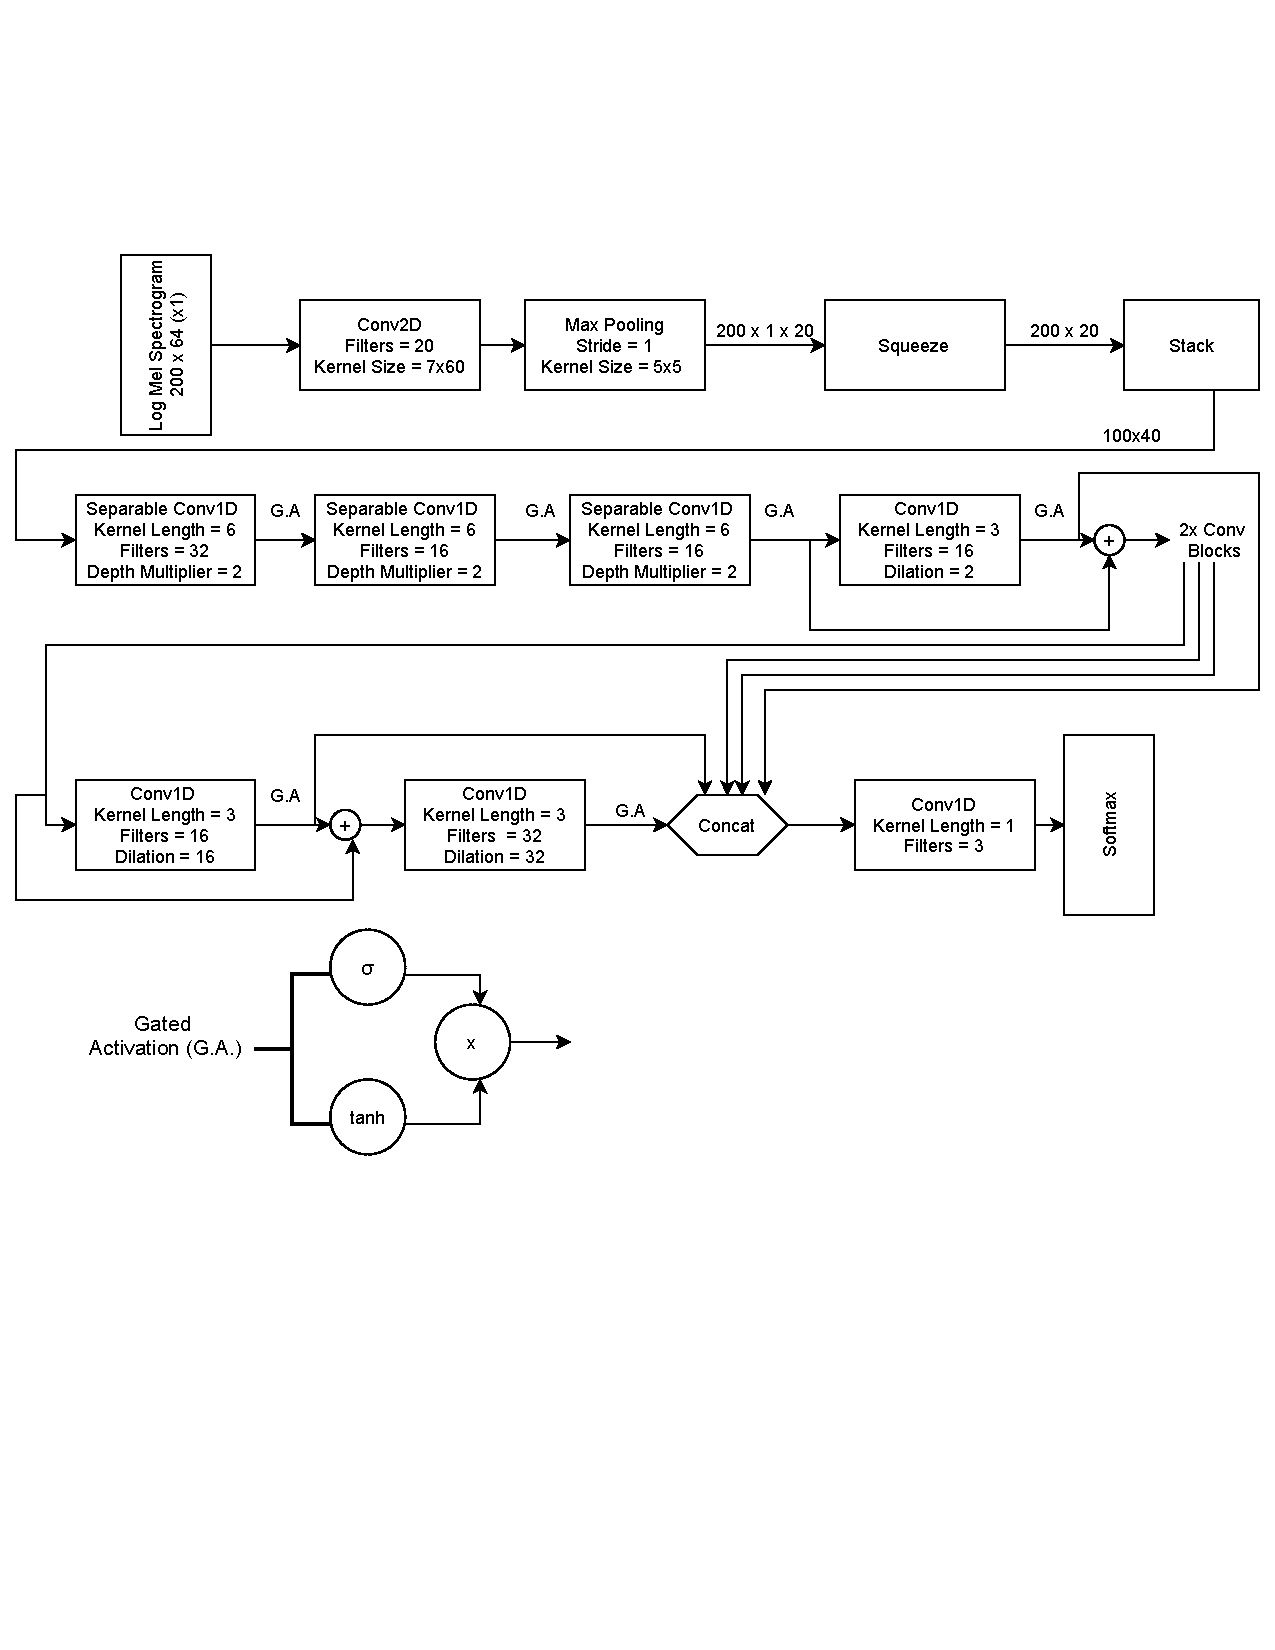
\includegraphics[width=\textwidth, trim= 0 230 0 100, clip]{Network.pdf}
	\caption{Network Architecture of SwishNet-slim}
	\label{fig:swishnet}
\end{figure*}

\begin{figure*}[!t]
	\centering
	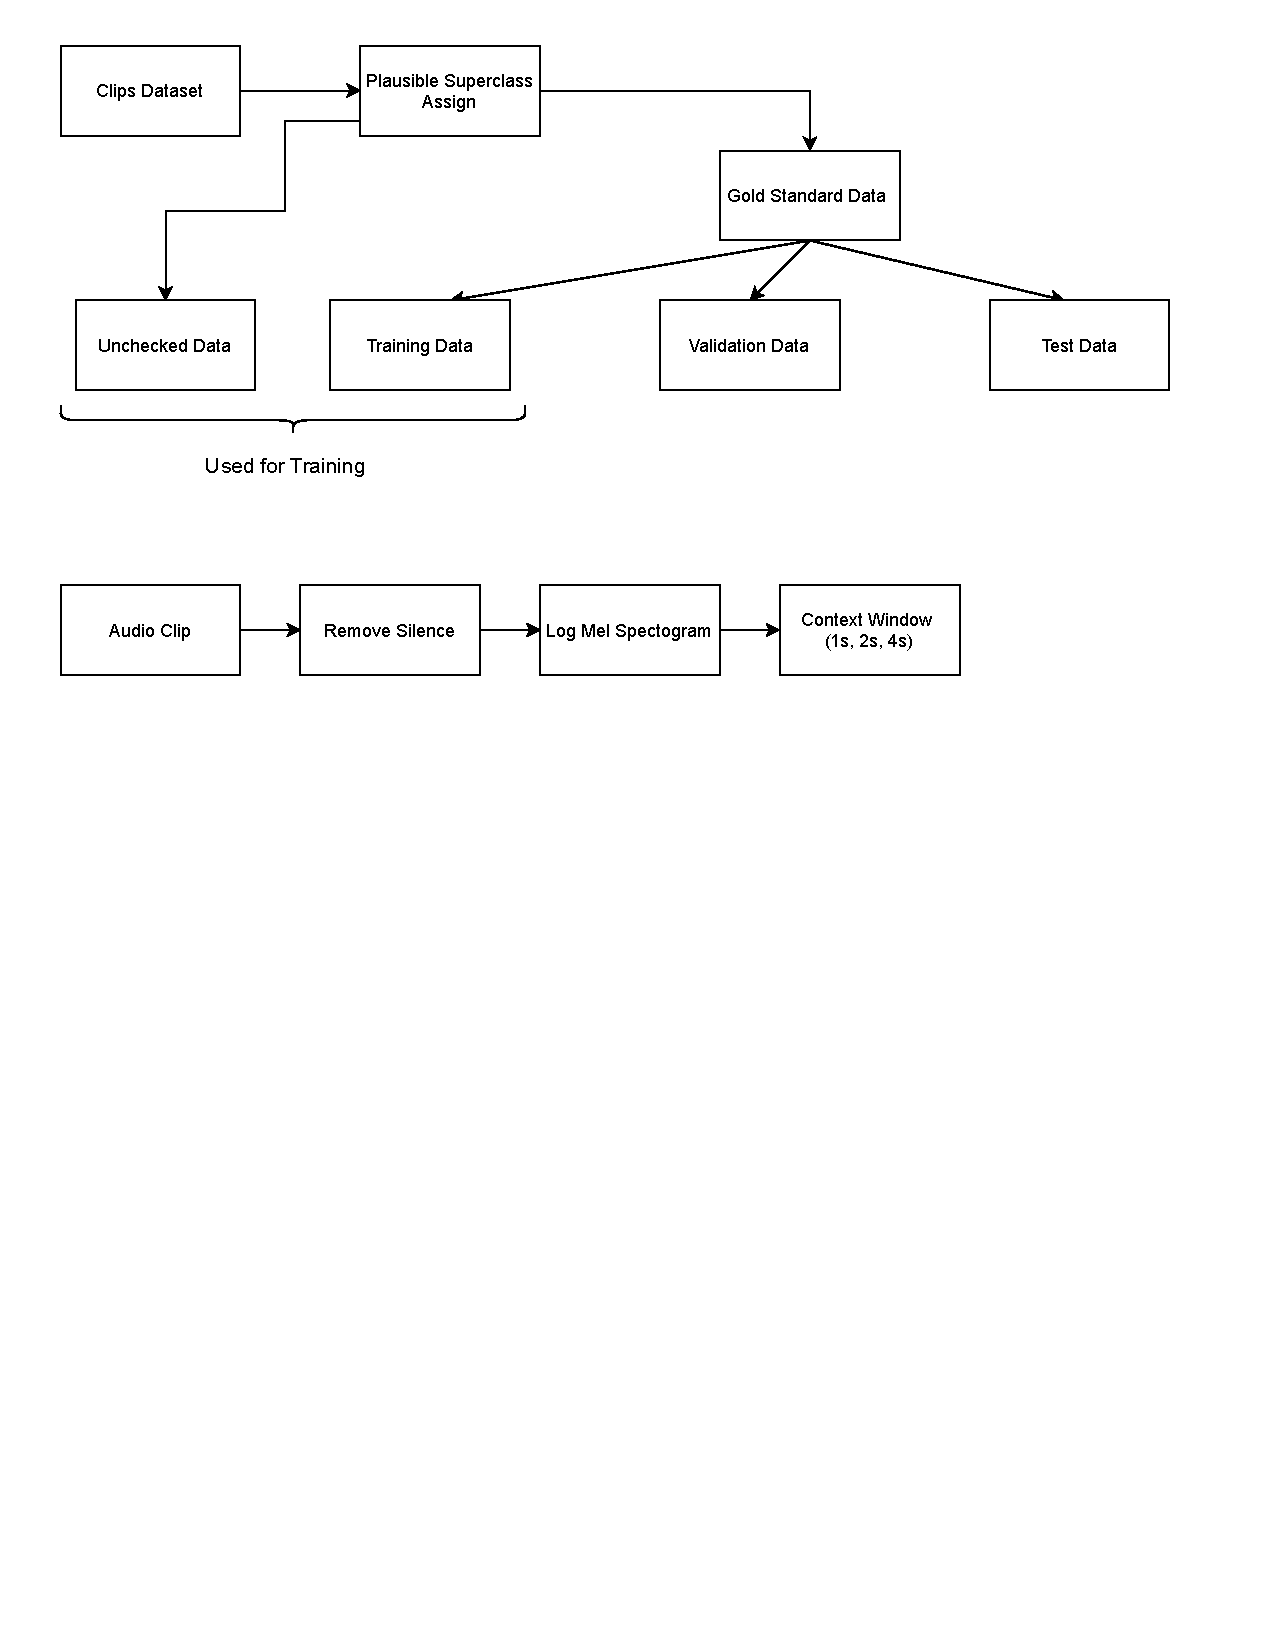
\includegraphics[width=\textwidth, trim= 0 450 0 0, clip]{Pipeline.pdf}
	\caption{Network Architecture of SwishNet-slim}
	\label{fig:swishnet}
\end{figure*}

\section{Related Works}
In general, audio content analysis in video parsing can be considered in two directions [5][6]. One is to discriminate audio streams into different classes such as speech, music, noise etc., the other is to classify audio streams into segments of different speakers. In this paper, our research work in the first direction will be presented. 

There have been many studies on audio content analysis, using different features and different methods [4] - 

Pfeiffer et al [1], presented a theoretic framework and application of automatic audio content analysis using some perceptual features. Saunders [2], presented a speech/music classifier based on simple features such as zero crossing rate and short time energy for radio broadcast. When a window size of 2.4s was used, the reported accuracy rate would be 98\%.  

Scheirer et al [3] introduced many more features into audio classification and performed experiments with different classification models including GMM (Gaussian Mixture Model), BP-ANN (Back Propagation Artificial Neural Network) and KNN (K-Nearest Neighbor). When using window of the same size (2.4s), the reported error rate would be 1.4\%. However, it is found that such simple features-based methods cannot work well when smaller window is used or more audio classes such as environment sounds are taken into consideration.  

Many other works have been done to enhance audio classification algorithms. In [7], audio recordings are classified into speech, silence, laughter and non-speech sounds, in order to segment discussion recordings in meetings. The accuracy of the segmentation resulted using his method varies considerably for different types of recording. In the work by Zhang and Kuo [8], pitch tracking methods are introduced to discriminate audio recordings into more classes, such as songs, speeches over music, with a heuristic-based model. Accuracy of above 90\% is reported. Srinivasan et al [5], try to detect and classify audio that consists of mixed classes, such as combinations of speech and music together with background sound. The accuracy of classification is over 80\%. 

\section{Methodology}

\subsection{Data Collection}
The Audioset [9] ontology was used to identify fine-grained sound event classes (source). We combined the fine-grained event classes into 3 major superclasses - speech, music and noise. We define each superclass uniquely by saying that a particular audio segment must not contain events from other superclasses, so that there is no ambiguity in classification. 

We downloaded the annotations of the YouTube video segments (source). Each segment is assigned multiple sound event tags. We defined plausible superclasses, based on these tags. If a clip contains only the subclasses of a given superclass (speech/music/noise) it is said to belong to that plausible superclass. If the superclass is ambiguous, we ignore that clip. But due to mistakes in annotations, missing annotations and human errors, the actual superclass may still be ambiguous or even wrong. So, the labels assigned at this point are noisy. 

Next, we downloaded YouTube clips in uncompressed wav format which was later compressed by the free lossless audio codec (FLAC). Clips were downloaded from the evaluation set, the balanced training set and the unbalanced training set. We downloaded about 81,000, 10s clips from YouTube.  

To generate ground truth (gold standard) annotations for the clips we manually checked each clip and verified their plausible superclass. If we found that a clip’s superclass was ambiguous, it was tagged as “bad”, otherwise it was tagged as “good”.  

We performed these manual annotations until we reached 4,000 clips for each superclass (speech, music, and noise). Thus, the gold standard (“good”) dataset contains 12,000 annotated unambiguous ground truth labeled clips. Also, the ambiguous (“bad”) labels are also kept for possible future use in automated label clean up. Our annotated dataset, along with unchecked clips is available publicly (source). 

\subsection{Feature Extraction}

\subsection{Network Architecture}

\section{Results and Discussions}



% Table generated by Excel2LaTeX from sheet 'Sheet1'

\begin{table}[!t]
	\centering
	\caption{Network Sizes and Prediction Times per Sample}
	\resizebox{\columnwidth}{!}{
		\begin{tabular}{p{4em}P{2.5em}ccccccP{3em}}
			\toprule[1pt]
			\multirow{4}[5]{4em}{\textbf{Network}} & \multicolumn{1}{c}{\multirow{4}[5]{2.2em}{\textbf{No. of Para-meters}}} & \multicolumn{6}{P{17em}}{\textbf{Prediction Time (ms) per Sample}} & \multirow{4}[5]{1cm}{\textbf{Weight file size}} \\
			
			\multicolumn{1}{p{1cm}}{} &       & \multicolumn{6}{P{17em}}{\textbf{for Different Sample Lengths}} & \multicolumn{1}{c}{} \\
			
			\cmidrule{3-8}    \multicolumn{1}{p{1cm}}{} &       & \multicolumn{2}{P{5em}}{\textbf{0.5s}} & \multicolumn{2}{P{5em}}{\textbf{1.0s}} & \multicolumn{2}{P{5em}}{\textbf{2.0s}} & \multicolumn{1}{c}{} \\
			
			\cmidrule(r{.25em}l){3-4} \cmidrule(r{.25em}l){5-6} \cmidrule(r{.25em}l){7-8}  \multicolumn{1}{p{1cm}}{} &       & \multicolumn{1}{p{1em}}{\textbf{CPU}} & \multicolumn{1}{p{1em}}{\textbf{GPU}} & \multicolumn{1}{p{1em}}{\textbf{CPU}} & \multicolumn{1}{p{1em}}{\textbf{GPU}} & \multicolumn{1}{p{1em}}{\textbf{CPU}} & \multicolumn{1}{p{1em}}{\textbf{GPU}} & \multicolumn{1}{c}{} \\
			
			\midrule[1pt]
			\textbf{GMM} & 92,416 & 1.8   & - & 3.6   & - & 7.2   & - & 370KB \\
			
			\midrule
			\textbf{SNN} & 179,203 & 0.71  & 0.72  & 0.92  & 0.72  & 1.52  & 0.82  & 717KB \\
			
			\midrule
			\textbf{SwishNet-slim} & 5,483 & 0.77  & 1.42  & 0.88  & 1.43  & 1.12  & 1.45  & 22KB \\
			
			\midrule
			\textbf{SwishNet-wide} & 18,267 & 0.9   & 1.45  & 1.1   & 1.45  & 1.65  & 1.45  & 66KB \\
			
			\midrule
			\textbf{MobileNet} & 217,235 & 4.1   & 3.51  & 5.27  & 3.52  & 8.57  & 3.55  & 870KB \\
			\bottomrule
		\end{tabular}
	}%
	\label{tab:speed}%
\end{table}%
\begin{table}[t]
	\centering
	\caption{Overall and Speech/Non-Speech (SNS) Classification Accuracy for Clips of Different Lengths}
	\resizebox{\columnwidth}{!}{
		\begin{tabular}{p{3em}p{4.1em}P{2.2em}P{2.2em}P{2.2em}P{2.2em}P{2.2em}P{2.2em}}
			\toprule
			\multicolumn{2}{p{8em}}{\textbf{Clip Length}} & \multicolumn{2}{M{6em}}{\textbf{0.5s}} & \multicolumn{2}{M{6em}}{\textbf{1.0s}} & \multicolumn{2}{M{6em}}{\textbf{2.0s}} \\
			
			\cmidrule(r{.25em}){1-2} \cmidrule(r{.25em}l){3-4} \cmidrule(r{.25em}l){5-6} \cmidrule(r{.25em}l){7-8} 
			\textbf{Network} &  & \textbf{Overall} & \textbf{SNS} & \textbf{Overall} & \multicolumn{1}{p{1.1em}}{\textbf{SNS}} & \textbf{Overall} & \textbf{SNS} \\
			
			\midrule[1pt]
			\textbf{GMM} &  & 96.53\% & 98.58\% & 97.33\% & 99.05\% & 97.79\% & 99.33\% \\
			
			\midrule
			\textbf{SNN} &  & 97.07\% & 98.87\% & 97.41\% & 99.13\% & 97.71\% & 99.36\% \\
			
			\midrule
			\multirow{2}{4em}{\textbf{Swish-Net-slim}} & \textbf{Undistilled} & 97.64\% & 99.24\% & 98.20\% & 99.60\% & 98.41\% & 99.76\% \\
			
			\cmidrule(l{0.5em}){2-8}          & \textbf{Distilled} & 97.52\% & 99.19\% & 98.22\% & 99.51\% & 98.57\% & 99.70\% \\
			
			\midrule
			\multirow{2}{4em}{\textbf{Swish-Net-wide}} & \textbf{Undistilled} & 97.97\% & 99.37\% & 98.32\% & 99.67\% & 98.65\% & 99.75\% \\
			
			\cmidrule(l{0.5em}){2-8}          & \textbf{Distilled} & 98.05\% & 99.45\% & 98.54\% & 99.71\% & 98.92\% & 99.84\% \\
			
			\midrule
			\multirow{2}{4em}{\textbf{Mobile-Net}} & \textbf{Random} & 98.13\% & 99.43\% & 98.53\% & 99.71\% & 98.95\% & 99.88\% \\
			
			\cmidrule(l{0.5em}){2-8}          & \textbf{Pretrained} & 98.94\% & 99.73\% & 99.24\% & 99.89\% & 99.38\% & 99.96\% \\
			\bottomrule
		\end{tabular}
	}%
	\label{tab:classperm}%
\end{table}%




\begin{table}
	\centering
	\caption{Normalized Confusion Matrices for Clips of Different Lengths (Rows: True Labels, Columns: Predicted labels, Ordering: Speech, Music, and Noise. GST = Trained on Gold Standard Training Set, GST + UT = Trained on Gold Standard and Unchecked Training Set, GST + UT + FT = Trained on Gold Standard and Unchecked Training Set, Fine Tuned on Gold Standard Training Set)}
	%\resizebox{\columnwidth}{!}{
	\begin{tabular}{M{13em}P{6.5em}P{6.5em}P{6.5em}} 
		
		\toprule
		\textbf{Network} & \textbf{1.0s} & \textbf{2.0s} & \textbf{4.0s} \\
		
		
		\midrule
		\textbf{SwishNet(GST)} 
		& $\begin{bmatrix}
		.90 & .05 & .05\\
		.02 & .92 & .06\\
		.02 & .11 & .86
		\end{bmatrix} $
		& $\begin{bmatrix}
		.93 & .03 & .03\\
		.01 & .94 & .05\\
		.02 & .11 & .87
		\end{bmatrix}$
		& $\begin{bmatrix}
		.93 & .03 & .03\\
		.01 & .94 & .05\\
		.03 & .11 & .86
		\end{bmatrix}$ \\
		
		\midrule
		\textbf{SwishNet(GST + UT)}
		& $\begin{bmatrix}
		.97 & .01 & .02\\
		.03 & .91 & .06\\
		.06 & .05 & .89
		\end{bmatrix}$ 
		& $\begin{bmatrix}
		.98 & .01 & .01\\
		.01 & .95 & .04\\
		.06 & .06 & 0.88
		\end{bmatrix}$
		& $\begin{bmatrix}
		.96 & .03 & .01\\
		.00 & .97 & .03\\
		.06 & .08 & .86
		\end{bmatrix}$\\
		
		\midrule
		\textbf{SwishNet(GST + UT + FT)} 
		& $\begin{bmatrix}
		.91 & .03 & .05\\
		.01 & .92 & .07\\
		.01 & .05 & .93
		\end{bmatrix}$ & 
		$\begin{bmatrix}
		.96 & .01 & .03\\
		.01 & .95 & .03\\
		.02 & .06 & .92
		\end{bmatrix}$ 
		& $\begin{bmatrix}
		.95 & .01 & .04\\
		.01 & .95 & .04\\
		.01 & .05 & .94
		\end{bmatrix}$ \\
		
		\midrule 
		\textbf{VGG16 (GST + UT + FT)} 
		& $\begin{bmatrix}
		.94 & .01 & .05\\
		.01 & .94 & .05\\
		.01 & .03 & .95
		\end{bmatrix}$ 
		& $\begin{bmatrix}
		.97 & .01 & .02\\
		.00 & .98 & .02\\
		.02 & .05 & .93
		\end{bmatrix}$ 
		& $\begin{bmatrix}
		.98 & .00 & .02\\
		.00 & .97 & .03\\
		.01 & .03 & .96
		\end{bmatrix}$ \\
		\bottomrule
	\end{tabular}
	%}
	\label{tab:conmat}%
\end{table}


\section{Conclusion and Future Work}


\printbibliography
\end{document}
